\documentclass[tikz,border=2pt]{standalone}
\usepackage{amsmath}
\usepackage{pgfplots}
\pgfplotsset{compat=1.18}
\usetikzlibrary{arrows.meta}
\begin{document}
% a=100, b=1, c=10: BR_1(q_2) = (90-q_2)/2 and BR_2(q_1) = (90-q_1)/2 (for quantities up to 90);
% the reaction lines cross once, at the Nash equilibrium (30,30).
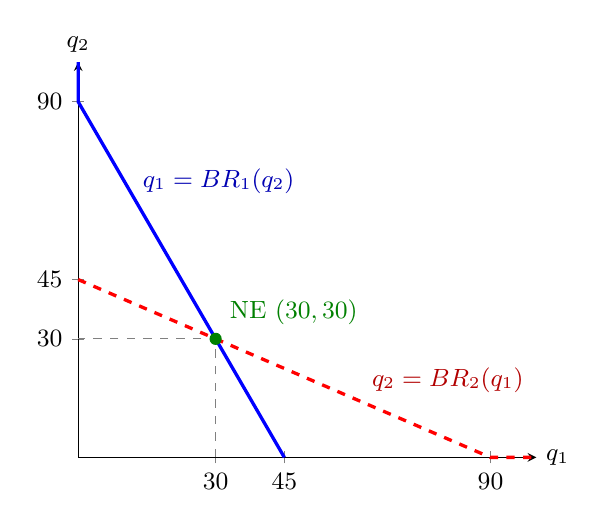
\begin{tikzpicture}[font=\small, >={Latex[length=2mm]}]
  \begin{axis}[
    axis lines=left,
    xmin=0, xmax=100, ymin=0, ymax=100,
    xtick={30,45,90}, ytick={30,45,90},
    xlabel={$q_1$}, ylabel={$q_2$},
    xlabel style={at={(axis description cs:1,0)}, anchor=west},
    ylabel style={at={(axis description cs:0,1)}, anchor=south, rotate=-90},
    tick label style={font=\small},
    samples=2, clip=false,
    width=7.4cm, height=6.6cm]
    % BR_1: q_1 = (90 - q_2)/2, from (45,0) to (0,90)
    \addplot[blue, very thick] coordinates {(45,0) (0,90) (0,100)};
    % BR_2: q_2 = (90 - q_1)/2, from (0,45) to (90,0)
    \addplot[red, very thick, dashed] coordinates {(0,45) (90,0) (100,0)};
    \node[blue!70!black, anchor=west] at (axis cs:12,70) {$q_1=BR_1(q_2)$};
    \node[red!70!black, anchor=south west] at (axis cs:62,14) {$q_2=BR_2(q_1)$};
    \draw[gray, thin, dashed] (axis cs:30,0) -- (axis cs:30,30) -- (axis cs:0,30);
    \fill[green!50!black] (axis cs:30,30) circle (2.2pt);
    \node[green!50!black, anchor=south west] at (axis cs:31,31) {NE $(30,30)$};
  \end{axis}
\end{tikzpicture}
\end{document}
